\documentclass[a4paper,11pt,twoside]{article}
\usepackage{amssymb}
\usepackage{hyperref}
\usepackage{booktabs}
\usepackage{geometry}
\usepackage{listings}
\usepackage{graphicx}
\usepackage{caption}
\usepackage{hyperref}
\usepackage{natbib}
\usepackage{todonotes}
\usepackage{enumitem}
\usepackage{multirow}
\usepackage{tikz}
\usepackage{fancyhdr}
\usepackage{xcolor,colortbl}
\usepackage{eurosym}
\usepackage{subfigure}
\usepackage[]{mcode}
\usepackage[page]{appendix}
\usetikzlibrary{arrows,decorations.pathmorphing,backgrounds,positioning,fit,petri,matrix,folding}

\setlength\headheight{20pt}
\addtolength\topmargin{-10pt}
\addtolength\footskip{20pt}

\newcommand{\HRule}{\rule{\linewidth}{0.5mm}}

\newcommand{\uni}{Eindhoven University of Technology}
\newcommand{\vak}{Database Technology}
\newcommand{\vakcode}{2ID35}
\newcommand{\essaytitle}{Smooth Scan Analysis}
\newcommand{\stad}{Eindhoven}
\newcommand{\tbsep}{\ \ \textbar \ \textbar \ \textbar \ \textbar \ \textbar \ \textbar \ \textbar \ \textbar \ \textbar \ \textbar \ \ }

\pagestyle{fancy}
\fancyhf{}
\fancyhead[RO,LE]{\vak}
\fancyhead[LO,RE]{\uni}
\fancyfoot[RO,LE]{\sffamily\bfseries\thepage}
\fancyfoot[LO,RE]{\essaytitle}
\renewcommand{\headrulewidth}{1pt}
\renewcommand{\footrulewidth}{1pt}

\bibliographystyle{plain}
\hypersetup{pdfborder={0 0 0}}

\setlength{\parskip}{10pt}

\geometry{
	includeheadfoot,
	margin=2.54cm
}
\author{
	Sander Breukink (0741209) - \texttt{s.c.breukink@student.tue.nl}\\
	Rianne Conijn (0740635) - \texttt{m.a.conijn@student.tue.nl}\\
	Harm van Schaaijk (0873871) - \texttt{h.a.h.v.schaaijk@student.tue.nl}\\
	Jasper Selman (0741516) - \texttt{j.w.m.selman@student.tue.nl}\\
	Tom Vogels (0871231) - \texttt{t.j.h.vogels@student.tue.nl}
}
\date{\today}

\begin{document}
	\begin{center} \thispagestyle{empty}

% Upper part of the page
		
\includegraphics[width=0.15\textwidth]{images/tuelogo}\\[1cm]

		\textsc{\LARGE \uni}\\[1.6cm]


        \textsc{\LARGE \vak}\\[0.5cm]

% Title
\HRule \\[0.4cm]
{ \huge \bfseries \essaytitle}\\[0.4cm]

\HRule \\[1.5cm]

% Author and supervisor
	\emph{Group number 25:}\\
    \begin{tabular}{l l l}
	Sander \textsc{Breukink} & 0741209 & \href{mailto:s.c.breukink@student.tue.nl}{\texttt{s.c.breukink@student.tue.nl}}\\
	Rianne \textsc{Conijn} & 0740635 & \href{mailto:m.a.conijn@student.tue.nl}{\texttt{m.a.conijn@student.tue.nl}}\\
	Harm \textsc{van Schaaijk} & 0873871 & \href{mailto:h.a.h.v.schaaijk@student.tue.nl}{\texttt{h.a.h.v.schaaijk@student.tue.nl}}\\
	Jasper \textsc{Selman} & 0741516 & \href{mailto:j.w.m.selman@student.tue.nl}{\texttt{j.w.m.selman@student.tue.nl}}\\
	Tom \textsc{Vogels} & 0871231 & \href{mailto:t.j.h.vogels@student.tue.nl}{\texttt{t.j.h.vogels@student.tue.nl}}
    \end{tabular}
		\vfill

% Bottom of the page
{\large \today} \\
\stad

	\end{center}

    \newpage
\begin{center}\section*{Abstract}\end{center}
In this paper a theoretical analysis of the \textit{Smooth Scan} algorithm \cite{smoothscan} is performed. The authors in this paper make several claims about their algorithm performing much faster than the often used \textit{Index Scan} and \textit{Full Scan} algorithms using new techniques. In this paper we will clarify these claims and compare \textit{Smooth Scan} with \textit{Index Scan}, \textit{Full Scan} and a combination of these two: \textit{Switch Scan}. Since there was unfortunately no source code or pseudo code of the \textit{Smooth Scan} algorithm availble, we used simulations instead of real verifying experiments. \\
In this paper we will first briefly state the problems which are discussed in the original paper, next summarize and explain the algorithms used in the paper and after that we will explain the verification plan for the analysis and discuss the results of the theoretical analysis.\\
We were able to replicate the nonrobust behavior of \textit{Switch Scan}. We were not able to completely replicate the behavior of \textit{Smooth Scan} as shown in the paper, but we show that this behavior strongly depends on the distribution of the data needed to be fetched.

\newpage
\section{Context and motivation}
Nowadays big data is booming business. A way to handle all this data in a fast efficient manner is very important for this cause. That is why at this time there are a lot of query optimizers, but these optimizers need statistics about the big data to create good query plans. The problem is that in many of these cases such statistics are sparse or even non-existent.

This is why Borovica, Idreas, Ailamakki, Zukowsku, and Fraser \cite{smoothscan} designed a new method for query optimizations decisions, the process of deciding which physical operators are used and in what order. Note that these decisions can affect the response time by several orders of magnitude and are therefore crucial in creating an optimally performing database. The authors propose a method called \emph{Smooth Scan} and its results are compared to those of a \emph{Full Table Scan}, an \emph{Index Scan} and a \emph{Switch Scan}. The \emph{Smooth Scan} is inspired by adaptive query processing, a technique which uses runtime feedback to modify query processing to get a better response time or more efficient CPU utilization \cite{query}.

The motivation for this article is the severe impact several scanning methods have on the total execution time, a response time which, in this day and age, becomes increasingly important. It also seems that the cost models for performance estimations deviate increasingly as the system becomes more complex. Combined with the fact that the complexity of modern workloads and the technological shift towards cloud environments, query optimization becomes increasingly important. Because of these reasons there is enough motivation to discuss a new scanning method for query handling.

\section{Research problem}
The main problem addressed in the paper is that once a decision is made by the query optimizer, this decision is fixed throughout the execution of a query. This can result in suboptimal plans and even a small estimation error can lead to drastically different performance results. These unpredictable results makes the system non-robust. The authors define robustness as: ``the ability of a system to efficiently cope with unexpected and adverse conditions, and deliver near-optimal performance for all query inputs.'' \cite{smoothscan} In their paper they try to achieve robust query processing.

\section{Smooth Scan}
In this section we briefly describe how the \emph{Smooth Scan} algorithm works. The former mentioned algorithms pick their strategy before the query is executed and stick to that strategy during the whole execution phase. The \emph{Smooth Scan} algorithm also picks a strategy at the start, but during the execution it might change strategy if necessary.

During the lifetime of \emph{Smooth Scan} the operator can be in three different modes. These modes are called \emph{Mode 1: Index Scan}, \emph{Mode 2: Entire Page Probe}, \emph{Mode 3: Flattening Access} and \emph{Mode 3+: Gradually Flattening Access}. In each of these modes the operator performs a gradually increasing amount of work as a result of the selectivity's increase.

In the first mode (in which \emph{Smooth Scan} always starts) a normal index scan is executed. Once the results cardinality threshold is exceeded it switches to mode 2. In this mode the operator performs a full page scan. If the result cardinality increases even more, \emph{Smooth Scan} changes to mode 3. In this mode the algorithm amortizes I/O cost over CPU cost (since you can do thousands of CPU operation during one I/O operation). This means the random selecting function is replaced with a sequential one. Mode 3+ is an expanded version of mode 3. Here the number of extra pages fetched for each single page it needs to access becomes larger and larger. Eventually this mode may change in a full table scan. For a more elaborate explanation of the algorithm we refer to section 3 of the work of Borovica et al. \cite{smoothscan}.

\section{Claimed results}
The authors implemented Smooth Scan in PostgreSQL and claim that it achieves robust performance in a range of synthetic and real workloads, while being statistics-oblivious at the same time. Existing approaches fail to do so. This robust behavior results in significant gains compared to when the original system makes a wrong decision, and only marginal overheads compared to when a correct decision can be made. Besides that, the authors also did the same tests with a SSD instead of a HDD. They claimed that SSD was even more beneficial for \emph{Smooth Scan} than HDD.

\section{Plan for verification}
During this project we want to verify the claims made in the paper by simulating the behavior of the \emph{Smooth Scan} in Matlab. First of all, the penalties for the index scan and full scan will be estimated. These estimations will be used to calculate the cost and thereby the execution time of the \emph{Full Scan} and \emph{Index Scan} for queries with different values of selectivity. Different properties of the database will be included and compared, such as clustered versus non-clustered data.

After this base situation is set up, we will simulate the behavior of the \emph{Switch Scan}, which will switch on set cardinality estimate. These results will be compared to the different established scenarios in order to verify the claims and key idea of the paper. We will conclude with the simulation of the \emph{Smooth Scan} and add these results to the comparison. Below we will describe the penalties used and assumptions made for each scan we will simulate.


\subsection{Index scan}
Since this scan is so well known, we will not elaborate how this scan works. The costs for the \textit{Index Scan} consist of two parts. The first part is traversing down the B+-tree, and the second one is fetching the pages. For a range query, the algorithm walks through the tree only once, this means it has one random I/O access to fetch the first page and for each next page in the query, the algorithm needs one sequential I/O access. For non-clustered data, the algorithm needs a random access I/O for each tuple. The costs for sequential search I/O's are significantly lower than for random search I/O's. At this point we assume that the penalty for a random I/O access is one to two orders of magnitude larger than the penalty for a sequential I/O access. This is in accordance with the original paper. The Matlab code for the simulation of the index scan can be found in Appendix \ref{appendixa}.

\subsection{Full scan}
The costs for the \textit{Full Scan} algorithm are quite easy to calculate. At the start we need one random I/O access to find the first page and from there on we need a sequential I/O access to fetch the next page. The algorithm keeps doing this until all the pages are fetched once. Again we use the same assumption for comparing random versus sequential I/O access. Next to I/O cost the algorithm also has a lot of CPU cost, because it needs to check for all tuples if they need to be selected. The Matlab code for the simulation of the full scan can be found in Appendix \ref{appendixb}.

\subsection{Switch scan}
To calculate the costs of this algorithm, we first need to explain briefly how this algorithm works. Before the algorithm starts it first calculates the expected selectivity. If the expected selectivity is very high it immediately starts with a \textit{Full Scan} and never switches. If the expected selectivity is low, it starts with the \textit{Index Scan}. Once the cardinality of the \textit{Index Scan} grows larger than the expected selectivity, the algorithm switches to a \textit{Full Scan} and throws away all results found so far. We also thought that it would be interesting to investigate how good the \textit{Switch Scan} would perform if we would swap the algorithms, such that it starts with a \textit{Full Scan} and once the real selectivity is so low that the expected selectivity can not be reached anymore, it switches to an \textit{Index Scan}. This extension is discussed in \autoref{sec:extension}.\\
The costs for the \textit{Switch Scan} are a combination of the costs of the previous two scans. If the selectivity is low, the costs of this scan is equal to the cost of the \textit{Index Scan} and when the selectivity is high it is equal to the costs of the \textit{Full Scan}.  Once the cardinality of the search exceeds a certain threshold, which is 0.01$\%$ of the data in our code, it stops with the index scan and continues  with the full scan. After this switch the total costs of the \textit{Switch Scan} is nearly double the value of the cost of the \textit{Full Scan}. This increase in time is caused by the time spent ineffectively on the \textit{Index Scan}. The Matlab code for the simulation of the Switch scan can be found in Appendix \ref{appendixc}.


\subsection{Smooth scan}
We tried to simulate the penalties of the \textit{Smooth Scan} based on the descriptions of the paper. We were not able to fully simulate the behavior, but we were able to make a good approximation. Our simulation starts in Mode 2, which is also known as the ''pessimistic'' approach in the paper. In Mode 2 we count the random page penalties for traversing the tree. When the current cardinality is higher then the set treshold for switching to Mode 3, the simulation will switch to Mode 3. Here the number of sequential page fetches, and thereby the sequential page costs is set on 200. When the current cardinality is higher then the set treshold for switching to Mode 3+, the simulation will switch to Mode 3+. Here the number of sequential page fetches will increase towards a full scan.

We set the cardinality treshold for switching to Mode 3 on \textbf{!!!TODO!!!} and to Mode 3+ on 0.005 times the number of tuples in the data. The Matlab code for the simulation of the Switch scan can be found in Appendix \ref{appendixd}.


\section{Verification results}
In this section we will discuss the results per simulated scan and compare these results. First we compared the \textit{Index Scan} with the \textit{Full Scan}. Thereafter we extended the results with the simulation of \textit{Switch Scan}. Finally we will evaluate the behavior of \textit{Smooth Scan}. For all simulations  we did a range query on a table with 1 million tuples, with 10 tuples per page. The tupples were non-clustered if not stated otherwise. \\

\subsection{Index Scan versus Full Scan}
\autoref{fig:result1} shows the penalties for different selectivity values for \textit{Index Scan} and \textit{Full Scan}. We tested different factors for the ratio, stating that the penalty for a random I/O access is 10, 20, 50, or 100 times larger than for a sequential I/O access. The penalty for sequential access is 10000 larger than for returning the tuple. \autoref{fig:result1} shows that for low selectivity, \textit{Index Scan} outperforms the \textit{Full Scan}. The higher the ratio, the lower the selectivity needs to be for the \textit{Full Scan} to outperform the \textit{Index Scan}. For a ratio of 10 the selectivity needs to be larger than 0.01, for a ratio of 20 the selectivity needs to be larger than  0.005, for a ratio of 50 larger than 0.002 and for a ratio of 100 even larger than 0.001.

Looking at the difference in selectivity you might notice that the increment of the ratio is the same as the decrement of the selectivity breakpoint for the  \textit{Full Scan} and \textit{Index Scan}. So we can clearly see that the ratio of the penalties of random access to the penalties of sequential access is important. Another important thing is that even in the most favorable scenario for this ratio (i.e. a ratio of 10:1 for random versus sequential access) the breakpoint for switching from an index scan to a full scan is already at a selectivity rate of 0.01 which is equal to a selectivity of 1$\%$. This is quite contradictory to the results found by Borovica et al. \cite{smoothscan}. They showed in a similar graph that the breakpoint is somewhere around the 14$\%$ selectivity. This is even in the best case about an order of magnitude difference. Borovica et al. claimed that the ratio of random to sequential access is somewhere in between 1 to 2 orders of magnitude, so if we look at the ratio of 100:1 we even see that we already reached the breakpoint at 0.1$\%$ selectivity. A reasonable explanation for this difference is that the DBMS system, PostgreSQL, has all kind of optimizations for the normal index scan. We do not have these optimizations and compare the penalties of the normal index scan to the full scan. 

Another interesting note is that Borovica et al. \cite{smoothscan} claim that the breakpoint for full scan and index scan lies somewhere between the 1 and 10$\%$ selectivity, but the graph, based on their results, shows a clear breakpoint of 14 to 15 $\%$. This is quite contradictory to what they claim and seems rather strange.

\begin{figure}[ht!]
\centering
\subfigure[Factor 10]{%
	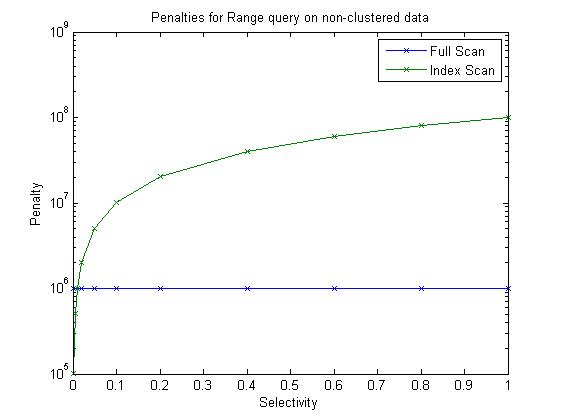
\includegraphics[width=0.45\textwidth]{images/Result2-Factor10}
	\label{fig:subfig1.1}}
\quad
\subfigure[Factor 20]{%
	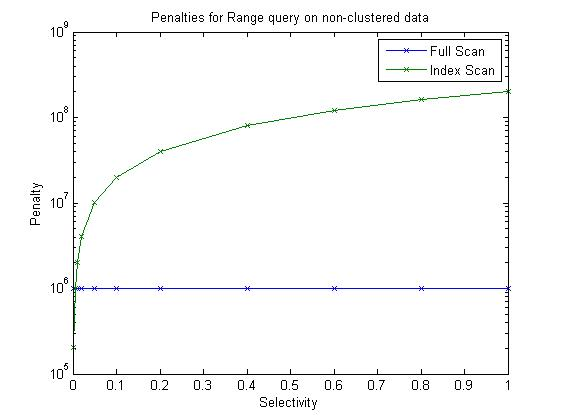
\includegraphics[width=0.45\textwidth]{images/Result1-Factor20}
	\label{fig:subfig1.2}}

\subfigure[Factor 50]{%
	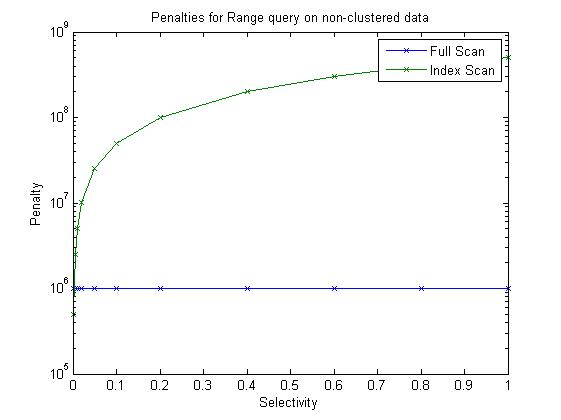
\includegraphics[width=0.45\textwidth]{images/Result3-Factor50}
	\label{fig:subfig1.3}}
\quad
\subfigure[Factor 100]{%
	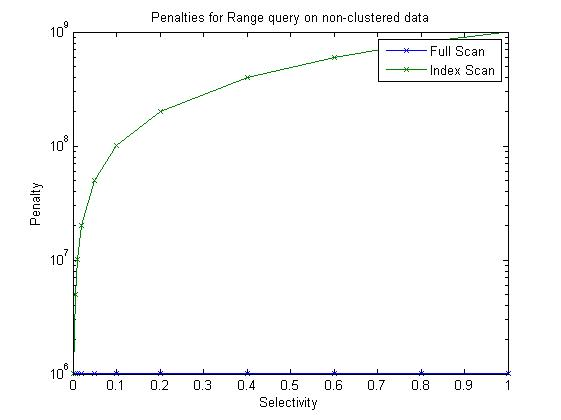
\includegraphics[width=0.45\textwidth]{images/Result4-Factor100}
	\label{fig:subfig1.4}}
%	
\caption{Penalties for \textit{Index Scan} and \textit{Full Scan} for a random query}
\label{fig:result1}
\end{figure}
%\pagebreak

\subsection{Switch Scan}
In this section we have extended the experiment with the \textit{Switch Scan} algorithm. The penalties for this algorithm are shown in \autoref{fig:result2}. In the upper two graphs we show the situation where the expected cardinality is 5 and 10$\%$. As you can see the interesting part of the graph lies at the most left side, that is the point where the \textit{Switch Scan} changes the algorithm. To study this part we have made the same graphs with a smaller range. These graphs are shown in Figure \autoref{fig:subfig2.3} and \autoref{fig:subfig2.4}.\\


\begin{figure}[ht!]
\centering
\subfigure[Cardinality of 5$\%$]{%
	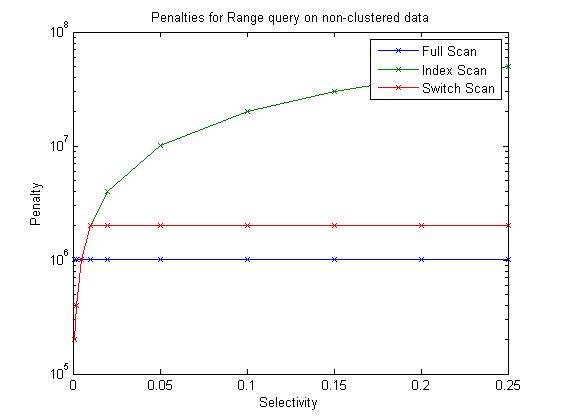
\includegraphics[width=0.4\textwidth]{images/Result5-Factor20-SwitchscanRandom}
	\label{fig:subfig2.1}}
\quad
\subfigure[Cardinality of 10$\%$]{%
	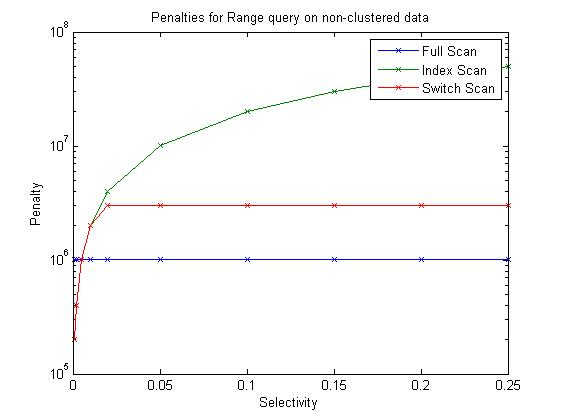
\includegraphics[width=0.4\textwidth]{images/Result5-Factor20-SwitchscanRandom-cardinality10perct}
	\label{fig:subfig2.2}}

\subfigure[Cardinality of 5$\%$ with a smaller range]{%
	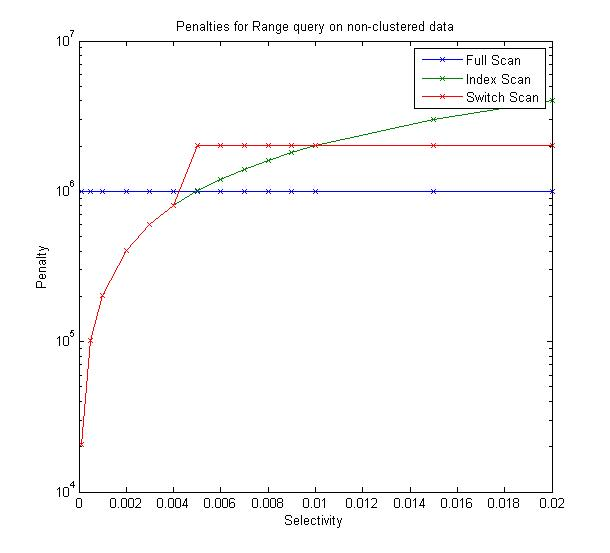
\includegraphics[width=0.4\textwidth]{images/Result6-Factor20-SwitchscanBeginloaded-cardinality5perct-02}
	\label{fig:subfig2.3}}
\quad
\subfigure[Cardinality of 10$\%$ with a smaller range]{%
	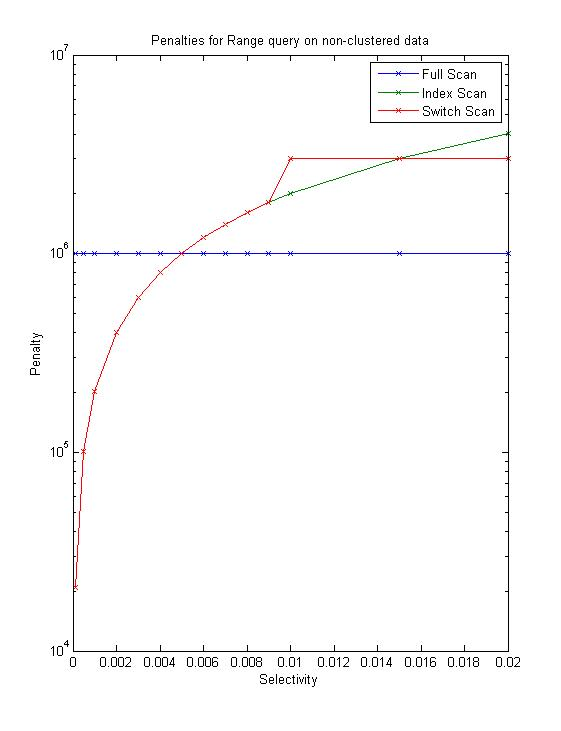
\includegraphics[width=0.4\textwidth]{images/Result6-Factor20-SwitchscanBeginloaded-cardinality10perct-02}
	\label{fig:subfig2.4}}
%		
\caption{Penalties for \textit{Switch Scan}, \textit{Index Scan} and \textit{Full Scan} for a random query}
\label{fig:result2}
\end{figure}
\pagebreak
As you can see in \autoref{fig:subfig2.3} there is a major spike in the number of penalties when the algorithm changes from \textit{Index Scan} to \textit{Full Scan}, especially when you note that the y-axis is in logarithmic scale. This is due to the fact that when \textit{Switch Scan} starts with a \textit{Full Scan}, all the results obtained so far with the \textit{Index Scan} are just thrown away. This is quite an issue, since the running time is two times longer than necessary when the real cardinality exceeds the expected cardinality. But if we look at the graph we see that \textit{Switch Scan} performs as good as the \textit{Index Scan} when the cardinality is expected lower than or equal to the breaking point of the two scans, which is at 0.5$\%$ for this dataset, and performs much better than the \textit{Index Scan} when the selectivity exceeds the 1$\%$. So this algorithm already works a lot better and is more robust than the \textit{Index Scan}, but a lot worse than the \textit{Full Scan} when the selectivity becomes higher. But this can be easily explained. In the way we implemented the \textit{Switch Scan} algorithm, it always starts with an \textit{Index Scan}, even if the expected selectivity is high. This is of course not logical for a real-life query optimizer and this optimizer will always start with a \textit{Full Scan} when the selectivity becomes higher than something near the 10$\%$.

The one small part where the \textit{Switch Scan} is worse than both algorithms is a real problem though. It looks like a very small range (only half of one percent), but in real-life the databases are huge and the result of the queries is very small compared to this database. This means that the selectivity of the tuples is indeed often very low. So a query might be often in this small range where \textit{Switch Scan} is worse than both \textit{Full Scan} and \textit{Index Scan}. This is especially the case when the found cardinality just slightly exceeds the expected cardinality as in this case the switching occurs very late in the database. This results in a performance-cliff at which both the \textit{Index Scan} and the \textit{Full Scan} are almost fully executed. This is of course undesirable yet may occur often when the optimizer's estimated cardinality is close to the real cardinality. The authors of the original paper acknowledged this problem and came with a solution for this. They created the \textit{Smooth Scan} algorithm, which has an extra mode next to just \textit{Index Scan} and \textit{Full Scan}. In the following section we will describe and evaluate our simulation of the \textit{Smooth Scan}.
%\pagebreak

\subsection{Smooth Scan}
Lastly, we extended the experiment with the \textit{Smooth Scan}. The penalties for this algorithm are shown in \autoref{fig:result3}. The \textit{Smooth Scan} was tested for three different distributions of the data in the dataset: random ordering of the tuples which need to be fetched, begin loaded, i.e., all important tuples are  at the beginning, and end loaded, i.e. all important tuples are at the end.

For randomly distributed tuples and low selectivities smooth scan works almost as good as index scan and switch scan. For larger selectivities, smooth scan is better than switch scan, but switch scan is even better. These results are worse than the results the paper found for the pessimistic approach of the smooth scan, where was found that smooth scan is much better than index scan. These worse results might be explained by ... \textbf{TODO}

However, for the cases where the important data is clustered, for example in the begin loaded and end loaded case, we find better results for smooth scan than in the paper. In these cases smooth scan outperforms index scan and full scan by far. This improvement in performance can be explained by the fact that in mode 2 of smooth scan the full page is fetched, and as the data is clustered, all the tuples on the page are important. Thus, it is very efficient that the whole page is fetched at once. 

\textbf{TODO WHAT ABOUT THE SPIKES IN C (I THINK SWITCHES TO MODE 3 AND MODE 3+ RESPECITVELY)}   
\begin{figure}[ht!]
\centering
\subfigure[Paper results]{%
	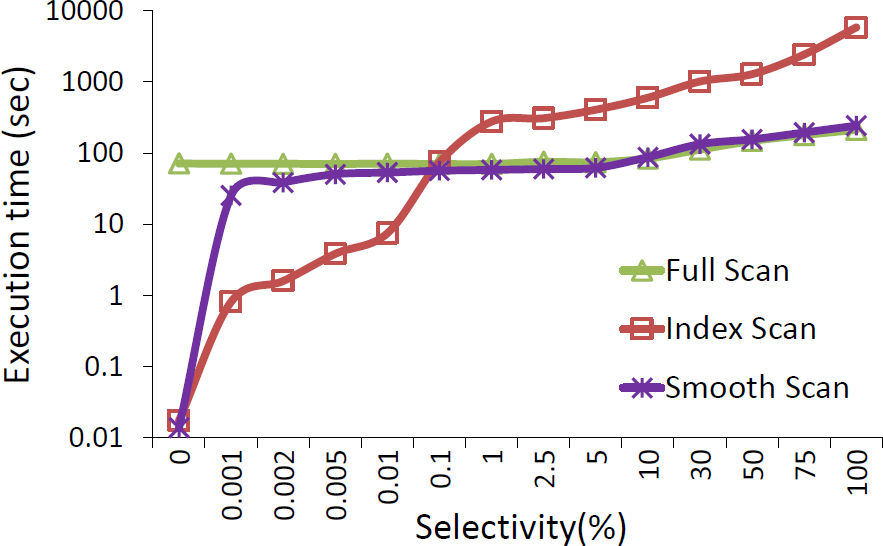
\includegraphics[width=0.4\textwidth]{images/theirresult}
	\label{fig:subfig3.1}}
\quad
\subfigure[Data randomly distributed]{%
	\includegraphics[width=0.4\textwidth]{images/Result8-Smoothscan-random-card05}
	\label{fig:subfig3.2}}

\subfigure[Data begin loaded]{%
	\includegraphics[width=0.4\textwidth]{images/Result8-Smoothscan-Beginloaded-card05}
	\label{fig:subfig3.3}}
\quad
\subfigure[Data end loaded]{%
	\includegraphics[width=0.4\textwidth]{images/Result8-Smoothscan-Endloaded-card05}
	\label{fig:subfig3.4}}
%		
\caption{Penalties for  \textit{Smooth Scan} \textit{Switch Scan}, \textit{Index Scan} and \textit{Full Scan} for a random query}
\label{fig:result2}
\end{figure}

\section{Extension of the paper}\label{sec:extension}
In the original paper, the authors implemented the \textit{Switch Scan} in such a way that it first starts with an \textit{Index Scan} and if it turns out that the expected selectivity was way too low, it switches to a \textit{Full Scan}. We thought that it was also interesting to see what happens in the other way around, so starting with the \textit{Full Scan} and switch to an \textit{Index Scan} when the optimizers estimate for the selectivity is too high. The results for this experiment are shown in \autoref{fig:result3}.

We have chosen for low values of the cardinality again, since the interesting part is in the switch part and since a lot of practical, real-life queries have low cardinality. As you can see in Figure \autoref{fig:subfig4.1} the graph looks very weird for the \textit{Switch Scan}, this is because it first executes a \textit{Full Scan}, but at the end of the full scan there are not enough tuples left to reach the expected level of cardinality and therefore the \textit{Switch Scan} algorithm switches to an \textit{Index Scan}. Though it looks like the \textit{Switch Scan} is only a bit above the line of the \textit{Full Scan}, this is already a lot worse, since the graph has a logarithmic scale on the y-axis.

As you can clearly see the algorithm never scores better than the \textit{Full Scan}algorithm. There is a good reason for that, namely it is useful to use an \textit{Index Scan} for selectivity ranges of 0$\%$ - 1$\%$ (according to our analysis) and for the rest a \textit{Full Scan}. Now when you start with a \textit{Full Scan} and the algorithm expects a cardinality of say 10$\%$, then the \textit{Full Scan} has completed its scan for already more than 90$\%$ before it realizes that the real selectivity rate is in fact (much) lower than the expected rate. Now it switches to an \textit{Index Scan} and starts over again. 

When you start with an \textit{Index Scan}, you do not have to complete the greatest part of the scan since it expects a low selectivity, if the optimizer was wrong than the low cardinality which is expected is quickly exceeded, so the algorithm changes to the \textit{Full Scan}. This makes it very logical that the \textit{Switch Scan} algorithm starts with the \textit{Index Scan} and that this option is not considered in the original paper.

\begin{figure}[ht!]
\centering
\subfigure[Cardinality of 0.5$\%$]{%
	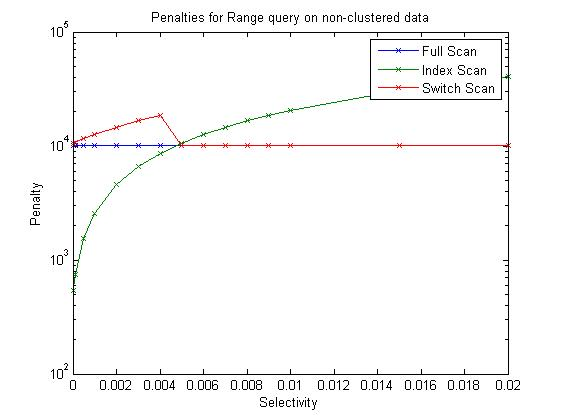
\includegraphics[width=0.4\textwidth]{images/Result7-Factor-SwitchscanFirstFull-Beginloaded-cardinality05perct}
	\label{fig:subfig4.1}}
\quad
\subfigure[Cardinality of 5$\%$]{%
	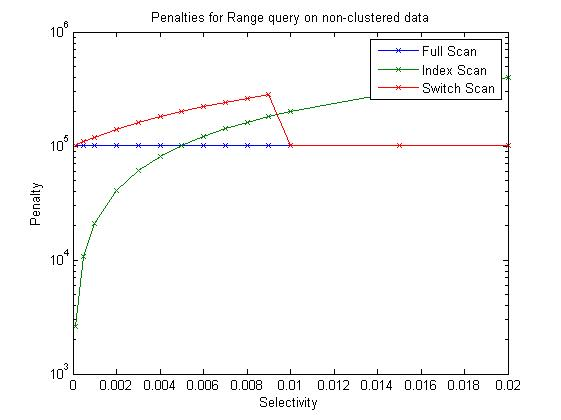
\includegraphics[width=0.4\textwidth]{images/Result7-Factor-SwitchscanFirstFull-Beginloaded-cardinality5perct}
	\label{fig:subfig4.2}}
%	
\caption{Penalties for \textit{Switch Scan} starting with a \textit{Full Scan} instead of a \textit{Index Scan}}
\label{fig:result3}
\end{figure}
\pagebreak

\section{Conclusion}
\textbf{HIER NOG EEN MOOI STUKJE VERTELLEN WANNEER SMOOTHSCAN AF IS OF WANNEER WE BESLOTEN HEBBEN DAT DIT NIET MEER LUKT.}

\begin{thebibliography}{9}

\bibitem{smoothscan}
	 Borovica, R., Idreos, S., Ailamaki, A., Zukowski, M., $\&$ Fraser, C.
	2015.	
 	Smooth Scan: One access path to rule them all.
	\emph{IEEE International conference on Data Engineering.}

\bibitem{query}
	Deshpande, A., Ives, Z., $\&$ Raman, V.
	2007.
	Adaptive query processing
	\emph{Foundations and Trends in Databases,}
	1(1), 1-140.
\end{thebibliography}
\newpage

\begin{appendices}
\section{Code index scan}
\label{appendixa}
\lstinputlisting{Simulation/IndexScan.m}
\section{Code full scan}
\label{appendixb}
\lstinputlisting{Simulation/FullScan.m}
\section{Code switch scan}
\label{appendixc}
\lstinputlisting{Simulation/SwitchScan.m}
\section{Code smooth scan}
\label{appendixd}
\lstinputlisting{Simulation/SmoothScan.m}
\end{appendices}

\end{document}
